\newcommand{\dpop}{\Delta p/p}

Изначальной целью экспериментов по изучению времени когерентности спина (Spin Coherence Time) на COSY было подтверждение возможности секступольных полей противодействовать дисперсии спин-тюнов, ассоциированной с 
эмиттансом и дисперсией импульсов ($\dpop$) частиц пучка.~\cite{COSY:SCT:IPAC15} На настоящий момент, оптимизация SCT является первой фазой любого предварительного эксперимента по поиску ЭДМ на COSY.

Секступольное подавление декогеренции используется совместно с электронным охлаждением пучка, для
уменьшения его фазового объёма, и банчингом, для подавления линейного вклада дисперсии импульсов частиц 
в декогеренцию. Секступоли, располагающиеся в арках, призваны подавлять эффект декогеренции второго порядка.

Для контроля декогеренции используются три семейства секступолей, которые маркированны соответственно: MXG, расположенный в максимуме дисперсионной функции, и контролирующий эффект декогеренции связанный с $\dpop$; MXS, расположенный в максимуме горизонтальной бета-функции $\beta_x$, и контролирующий дисперсию, связанную с горизонтальными бетатронными колебаниями; MXL, в максимуме $\beta_y$, контролирующий дисперсию, возникающую из-за вертикальных бетатронных колебаний.

\begin{figure}[h]\centering
	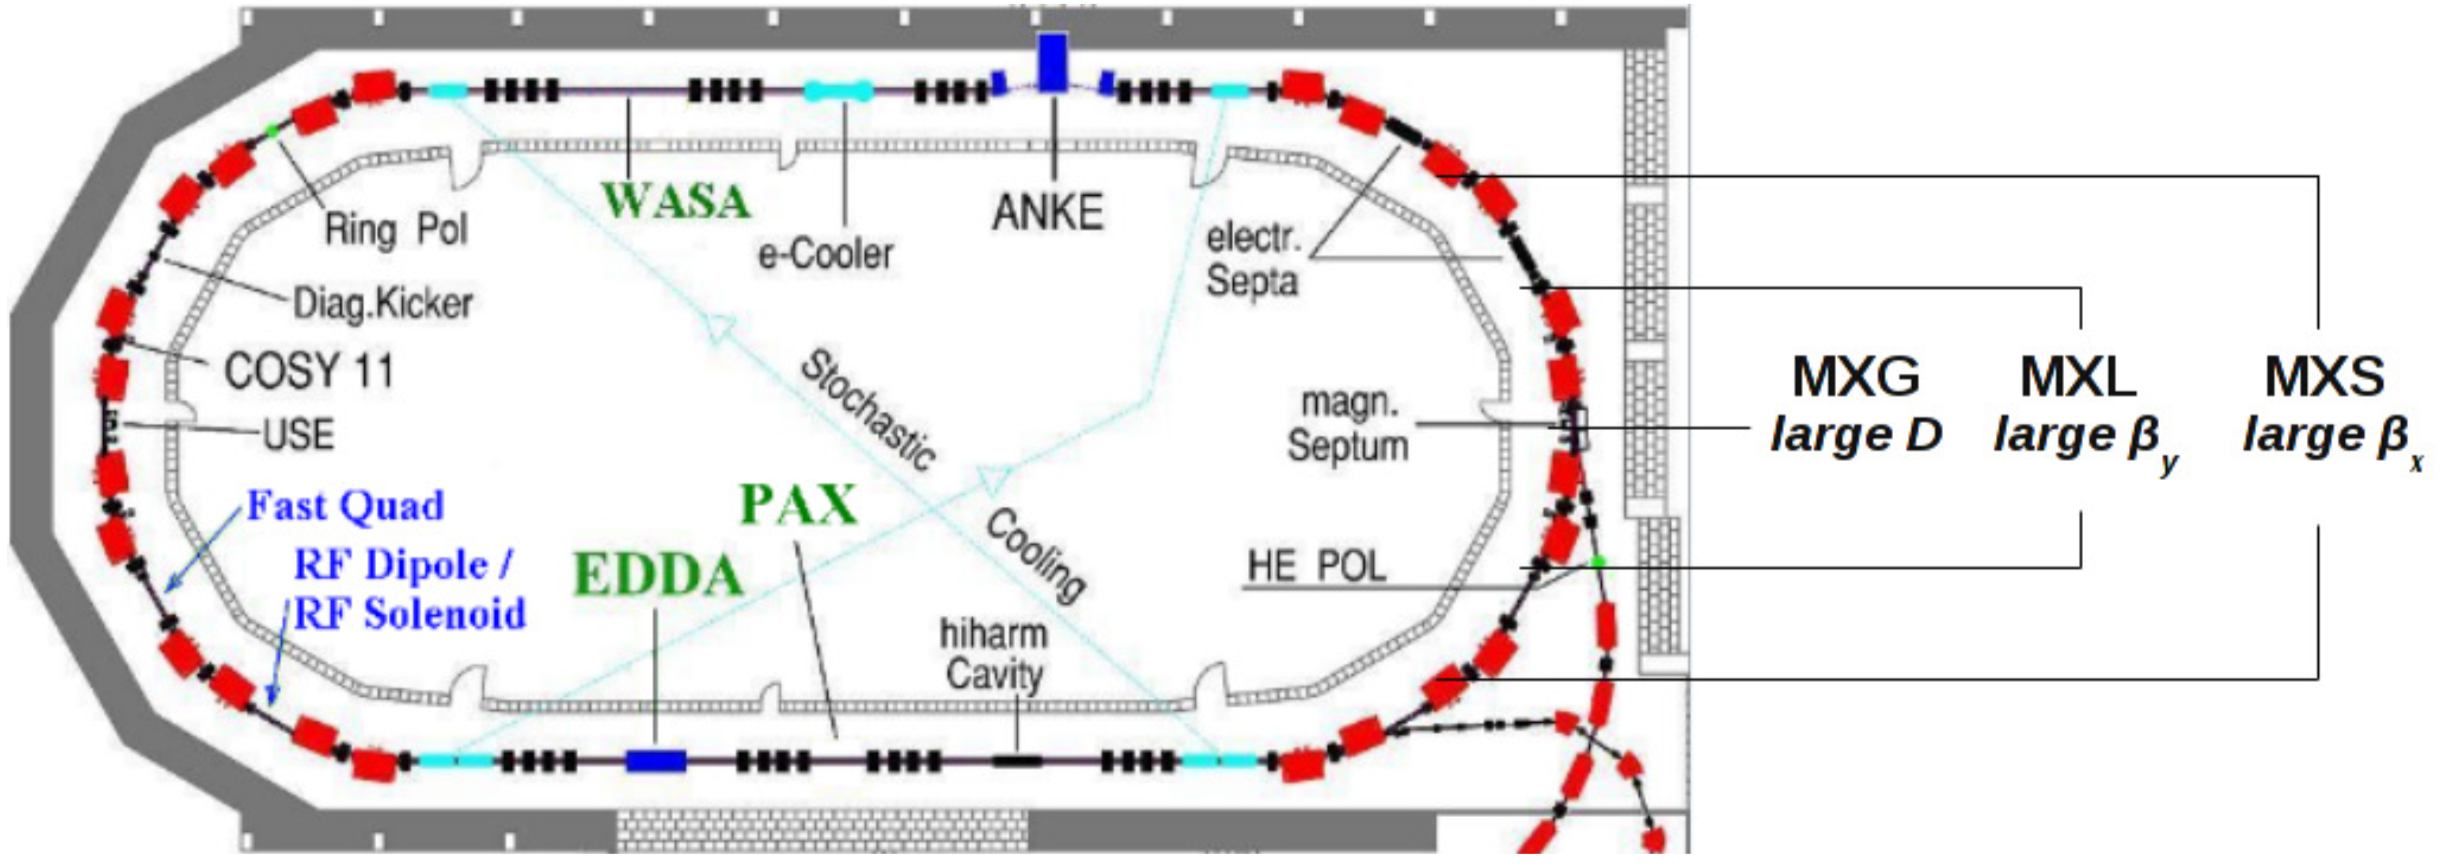
\includegraphics[width=\linewidth]{images/chapter4/COSY-sextupoles}
	\caption{Кольцо COSY с отмеченными положениями секступолей для контроля времени когерентности спина. (Рисунок взят из~\cite{Guidoboni:STORI14}.)}
\end{figure}

\subsection{Процедура оптимизации}
В этом разделе описана процедура оптимизации SCT, на примере эксперимента 2014 года.~\cite{Guidoboni:STORI14} Первый оптимизационный эксперимент проводился в 2012 году, но тогда варьировалась только напряжённость поля секступоля MXS. В 2014 году впервые проведён полноценный (варьировались градиенты всех трёх секступолей) эксперимент по оптимизации SCT. 

Чтобы отделить эффекты декогеренции, связанные с конечностью эмиттанса пучка, и с вторым порядком дисперсии импульсов частиц $(\dpop)^2$, подготовка пучка к эксперименту проводится по-разному.

Для получения пучка с большим разбросом $(\dpop)^2$, поляризованный дейтронный пучок с импульсом $p=0.97$ ГэВ/с сначала охлаждается в течении 60 секунд для минимизации его эмиттанса. После отключения охлаждения пучок банчируется (гармоническое число $h=1$). Банчирование необходимо для подавления линейных эффектов декогеренции.

В случае изучения декогеренции, связанной с горизонтальным эмиттансом пучка,~\footnote{Декогеренция, связанная с вертикальным эмиттансом не может быть изучена ввиду ограничений по аксептансу.} охлаждение и банчирование проводятся одновременно в течении первых 60 секунд, после чего охлаждение отключается, и на пять секунд включается горизонтальное нагревание. Пучок нагревается подачей белого шума на обкладки конденсатора горизонтального кикера.

В обоих случаях, пучок инжектируется с вертикально-ориентированным вектором поляризации. Поворот поляризации в горизонтальную плоскость производится ВЧ соленоидом, после подготовки пучка, на 80-й секунде.

Мониторинг поляризации пучка производится непрерывно, путём приложения белого шума на вертикальный кикер, для экстракции пучка на 17-мм углеродную мишень. Далее, эластично-рассеянные дейтроны детектируются на поляриметре EDDA. Эластичное рассеяние дейтронов на углеродной мишени чувствительно к направлению спина, и имеет большое сечение взаимодействия. 

Сцинтилляторы поляриметра поделены на четыре группы: верхние, нижние, левые, правые; асимметрия частот событий на левом и правом детекторах пропорциональна вертикальной поляризации, а на верхнем и нижнем --- горизонтальной поляризации. Прецессия поляризации пучка в горизонтальной плоскости происходит с частотой, значительно превышающей частоту выборки поляриметра, поэтому в 2012 году была разработана специальная система сбора данных~\cite{COSY:SCT:DAQ}.

По результатам эксперимента~\cite{Guidoboni:STORI14} была доказана возможность получать на COSY SCT свыше 1,000 секунд. 

\subsection{Изменение SCT при переходе от внешней к внетренней части пучка}
Ниже представлены результаты оптимизации SCT, полученные в период измерений апрель-май 2019 года. 

На серии рисунков~\ref{fig:April2019:Polarization} представлены измерения асимметрии частоты событий на левом и правом детекторах (так называемая асимметрия лево-право), которая пропорциональна вертикальной компоненте поляризации пучка. На первых двух рисунках можно наблюдать, что на начальном этапе (в промежутке от 100 до 150 секунд) деполяризация происходит со значительной скоростью, но во второй половине цикла скорость деполяризации падает. На Рисунке~\ref{fig:Polariation:recovery-from-halo-to-core} особенно, мы видим, что в промежутке времени приблизительно от 130 до 150 секунд поляризация начинает возрастать, прежде чем снова спадает со значительно меньшей скоростью.
\begin{figure}[h]\centering
	\subbottom[SCT = $20.87 \pm 1.49$ секунд.\label{fig:Polariation:recovery-from-halo-to-core}]{%
		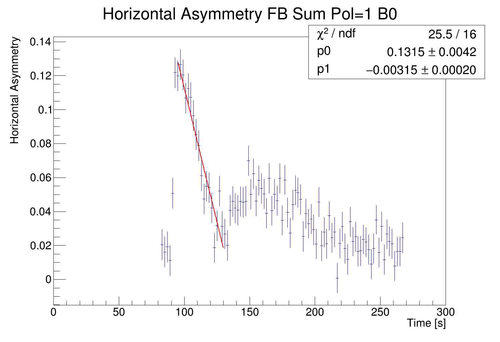
\includegraphics[height=.35\paperheight]{images/chapter4/SCT-April-2019/11th_19-55}}
	\subbottom[SCT = $42.3 \pm 2.2$ секунд.]{%
		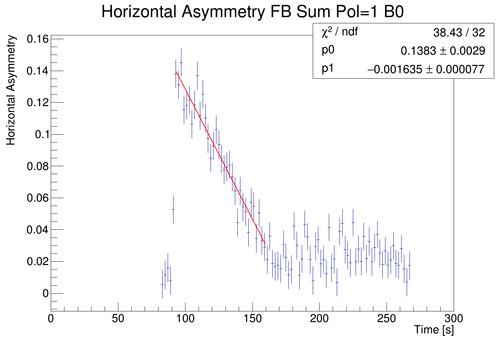
\includegraphics[height=.35\paperheight]{images/chapter4/SCT-April-2019/11th_20-20}}
\end{figure}
\begin{figure}[h]\centering
	\contsubbottom[SCT = $70.6 \pm 4.1$ секунд.\label{fig:Polarization:halo-and-core-similar}]{%
		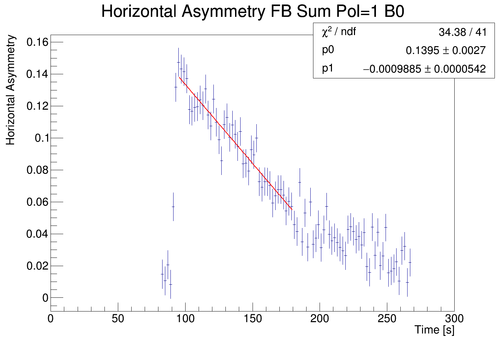
\includegraphics[height=.35\paperheight]{images/chapter4/SCT-April-2019/11th_20-31}}
	\contsubbottom[SCT = $302.0 \pm 27.5$ секунд.]{%
		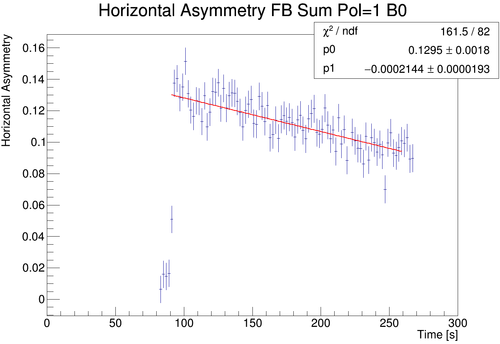
\includegraphics[height=.35\paperheight]{images/chapter4/SCT-April-2019/13th_03-23}}
	\caption{Измерения вертикальной поляризации во время оптимизации времени когерентности спина при подготовке к эксперименту по поиску аксионов в Апреле 2019 года.\label{fig:April2019:Polarization}}
\end{figure}

Такое поведение поляризации на данный момент объясняется неоднородностью поляризованности пучка. В первой половине цикла на детектор преимущественно попадают частицы из внешней (halo) части пучка (оболочки); к второй половине цикла начинается выборка частиц из центральной (core) части (ядра). Поскольку ядро плотнее чем оболочка, вариация длин орбит частиц ядра меньше, чем частиц оболочки, а значит меньше и разброс спин тюнов частиц.

\begin{figure}[h]\centering
	\subbottom[Секступоль MXL.]{%
		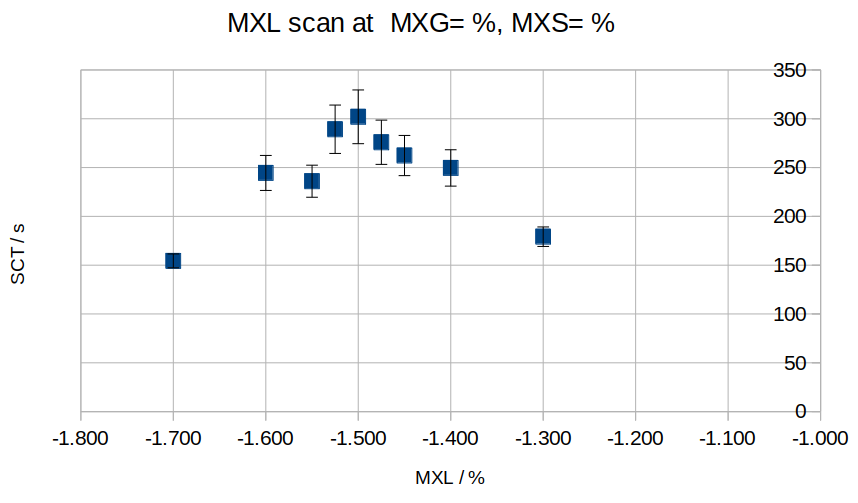
\includegraphics[height=.35\paperheight]{images/chapter4/SCT-April-2019/MXL_scan}}
	\subbottom[Секступоль MXG.]{%
		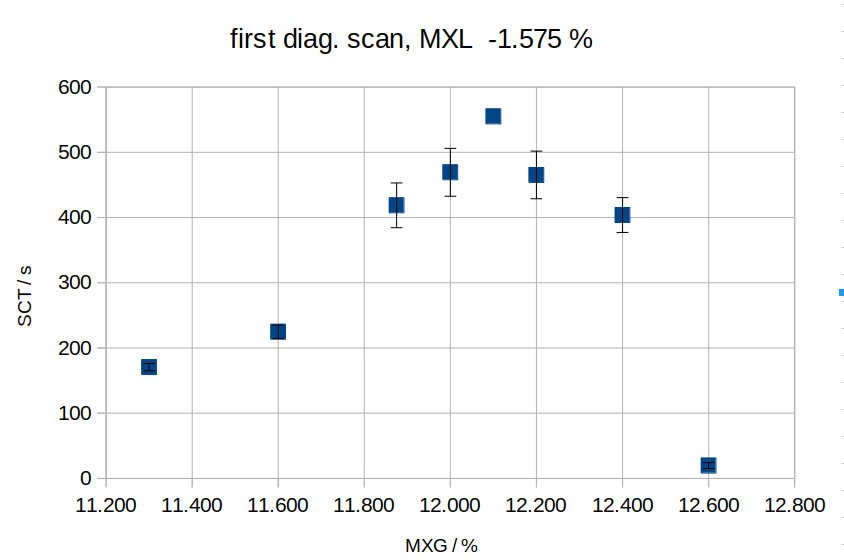
\includegraphics[width=.6\paperheight]{images/chapter4/SCT-April-2019/MXG_scan}
	}
	\caption{Зависимость SCT от градиента секступоля.\label{fig:SCT_scan}}
\end{figure}

На Рисунках~\ref{fig:SCT_scan} представлена зависимость времени когерентности спина от относительной силы поля, соответственно MXL и MXG секступолей.